\section{Language for Speculation}\label{sec:language}

In this section, we define a language for speculation -- its syntax and
operational semantics. We also present illustrative examples.
% We start out by presenting the data model which is independent of the rest of the language.
% Then we describe the syntax and the operational semantics of the language,
% and finally we discuss the exit and commit semantics along with some examples
% to help understanding of the language.

\subsection{Data Model}\label{sec:datamodel}

In speculative nondeterminism, we assume a 
centralized data store acting as the primary programming environment. The implementation of this store is
not part of the language and therefore independent from the operational semantics of the language.
Here we present the abstract data model of the store that can be instantiated into different
concrete models.

A data model is a 6-tuple
$$\dm=\langle D_0,\alltype,\allop,\allstore,\vdash,\psi\rangle$$
where
\begin{description}
  \item[$D_0$] defines an empty data store, for example, 
    an empty set $\emptyset=\{\}$ or an empty multi-set $\lbb\rbb$.
  \item[$\alltype$] is the set of all possible data items in the data model.
    For example, $\alltype=\nat$ for data models such as a set of natural numbers. 
  \item[$\allop$] is the set of all data operations available in the data model.
  \item[$\allstore$] is the set of all possible data stores.
    For example, $\allstore=2^\nat$ for data models such as a set of natural numbers.
  \item[$\vdash\subseteq\allstore\times\allop$] is a binary relation denoted by $D\vdash d$.
    It defines when operation $d$ can be executed on the data store $D$.
    For example, if the operation $d$ has a precondition, $D\vdash d$ is
    true if and only if the condition is true when evaluated on the data store $D$.
  \item[$\psi:\allop\times\allstore\to\alltype\times\allstore$] is the transition function that
    defines the effect of data operations on the store. 
    In general, a data operation can do read, update, or both. 
    For read purpose, a data item $t\in\alltype$ in the data store must be returned from $\psi$. 
\end{description}

Next we give some examples of concrete data models under the above framework.

\subsubsection*{Tuple Space}

The idea of tuple space comes from Linda \cite{Gelernter85:Linda}, where
a tuple space is a multi-set of tuples that can be accessed concurrently.
A tuple is an ordered collection of fields. 
Agents can post their data to the tuple space in the form of tuples, and 
retrieve tuples as data from the tuple space that match a certain pattern.
There are three major operations in the tuple space data model:
(i) $\In$ reads and removes a tuple from a tuple space;
(ii) $\Out$ produces a tuple, writing it into a tuple space;
(iii) $\Rd$ non-destructively reads a tuple space and gets a copy of a tuple. 
Both $\In$ and $\Rd$ are blocking while $\Out$ is non-blocking.
Formal definitions and operational semantics for
the $\In/\Out/\Rd$ operations \cite{Ciancarini95}
can be easily adapted to this framework.

\subsubsection*{Key-value Store}

{\em Key-value store} is a mapping from keys 
to values, e.g.
$[a\mapsto 3, b\mapsto 5]$ is a key-value store
where the key $a$ gets value $3$ and $b$ gets $5$.
Typical data operations include: (i) creating a new key-value pair,
(ii) updating an existing key with a new value,
(iii) getting a value according to a key, and
(iv) removing a key and its corresponding value.
Conditional guards can also be combined with these data operations,
e.g., $a>4\Rightarrow b\gets 2$ waits (blocks) until
the condition $a>4$ is true in the store,
and then updates the value of $b$ to $2$.

\subsubsection*{Other Models}

Other more structured data models include relational data and logic programs.
Data operations are insertion and deletion of tuples/predicates. Applications
using these models are also typical.


\subsection{Syntax}\label{sec:syntax}

% \RY{explain syntax, examples and then semantics. The semantics needs to
% be more detailed in the explanation and motivate the definitions etc.,
% e.g. what does commit do, what is the effect of this particular commit.
% What does exit do - why not just exit immediately. Also commit and
% exit are not immediate, again this is because of what they do.
% The local transitions part seems messy with things which are not defined
% but used. \\
% Erlang style notation has to be briefly explained. Use the first
% 2 rules in fly for this.
% }

\begin{figure}
\centering
\begin{eqnarray*}
     \text{Agent } a & := & p:f ~~|~~ \exiting ~~|~~ \exited \\
   \text{Program } p & := & e ~~|~~ op.e ~~|~~ t.e ~~|~~ e_1.e_2 ~~|~~ \epsilon \\
\text{Operation } op & := & d ~~|~~ e_1\oplus e_2 ~~|~~ \cm ~~|~~ \cu ~~|~~ \exit \\
                     &    & \\
      \text{Tree } T & := & w ~~|~~ T_1\oplus_k T_2 \\
     \text{World } w & := & \langle A,D,S\rangle \\
    \text{Agents } A & := & [] ~~|~~ [a_1,\dots,a_m] \\
 \text{Snapshots } S & := & \emptyset ~~|~~ \{s_1,\dots,s_n\} \\
  \text{Snapshot } s & := & \langle k,v\rangle
\end{eqnarray*}
\caption{Syntax and Runtime Data Structures.
$f:\allstore\to\nat$ is a exit function.
$e$ denotes a local computation,
$t\in\alltype$ is the input for the local computation,
and $\epsilon$ is the end of a local computation.
Dot (.) in $p$ means sequencing.
$d\in\allop$ is a data operation while $D\in\allstore$ is a data store.
$k\in\nat$ is the identifier of an agent.
$v\in\nat$ is an exit value of an agent.
}\label{fig:syntax}
\end{figure}

The syntax of the language for speculation is 
formally described in Figure \ref{fig:syntax}. 
The idea is that we have two languages, one which deals with the speculative
computation, the other is a host language where the speculation constructs
are embedded within.
The host and speculation language are conceptually orthogonal though
in practice one would want them to be closer.
In our syntax, an agent consists of a program $p$ and an exit function $f$. 
In the syntax in Figure \ref{fig:syntax}, $e$ is used to denote a language
computation in the host language. Since the host language is arbitrary, we
only define a meta syntax here\footnote{
The syntax here is similar to \cite{Ciancarini95} which gives a semantics
of Linda embedded in a host language.
}
in that $e$ is meant to evolve to some other
local computation $e'$ outside our semantics.
We use $\epsilon$ to denote the end of such a local computation. 
There is a special syntax $t.e$ where $t$ is intended to be the
result of the data operation $d$ ($t$ is the result of transition function $\psi$).
The meaning is that $e$ is intended to consume the result $t$, which overloads,
the dot symbol.\footnote{
This is because $d$ is defined in the data model but divorced from the host
language, thus, there would be something in the host language to deal with
the result $t$.
}
During runtime, an agent can also switch to special states $\exiting$ and $\exit$, 
which will be explained in Section \ref{sec:semantics}. 

The top-level runtime data structure is the tree of worlds,
while a world is a triple of a list of agents $A$, 
a data store $D$, and a set of snapshots $S$. 
A snapshot $s=\langle k,v\rangle$ is used in exit 
where $k$ denotes the $k$-th agent and $v$ is the exit value. 
%

\begin{figure}[tb]
\begin{lstlisting}[caption={Speculation Example using Tuple Space. 
We use \texttt{(...)} to denote tuples and
$\lambda x.\varphi(x)$ denotes a condition for $\In$ and $\Rd$ on the specific field in a tuple, where $\varphi$ is the condition expression such as ``$x\texttt{=ac}\lor x\texttt{=cb}$'' which means $x$ is equal to either {\tt ac} or {\tt cb}.},label=lst:ts-example]
|$\In$|(ticket, ab)
|$\oplus$|
(|$\In$|(ticket, |$\lambda x.x\texttt{=ac}\lor x\texttt{=cb}$|) = (ticket, X)
 if X = ac
   |$\In$|(ticket, cb)
 else
   |$\In$|(ticket, ac))
\end{lstlisting}
\end{figure}

We use the tuple space data model throughout this paper 
due to its simplicity and expressive power.
In order to explain further, we rewrite Listing \ref{lst:intro-speculate}
concretely using the tuple space data model and show it in Listing \ref{lst:ts-example}.
%
We use this style of host language from now on to 
demonstrate local computations as well as to embed speculation primitives, where
(i) identifiers starting with lowercase letters are symbol literals,
(ii) identifiers starting with uppercase letters are variables,
(iii) equal sign (\texttt{=}) denotes pattern matching and binding,
(iv) variables are immutable after binding,
(v) $\lambda x.\varphi(x)$ is a first-class anonymous function 
taking $x$ as the parameter and evaluating $\varphi(x)$ as 
the result of the function on calling. 
%\KZ{But what's $x$? Its type?} 
Such features are derived from functional languages such as Haskell and Erlang. 
The choice of host language is primarily for ease of presentation,
since the speculative nondeterminism framework is independent of 
the host language and local computations.
However, we also have a prototype implementation in Erlang which also uses
Erlang as the host language, thus our syntax is most similar to Erlang.


\subsection{Examples}\label{sec:examples}

Next we describe some examples to help understanding the language.
% \XJ{TODO: exit function f inside at least one example}

% \subsubsection*{Bob and Jill (BJ)}

This example is about trading in an online marketplace. 
Photographer Bob wants to upgrade his equipment while Jill wants to downgrade.
Bob can either buy good lens and sell his average lens, 
or buy a good camera and sell his average camera.
Jill can either sell her good lens and buy an average camera, 
or sell her good camera and buy an average camera.
Listing \ref{lst:bob} and \ref{lst:jill} show the 
agent programs of Bob and Jill, respectively.
Both \texttt{buy()} and \texttt{sell()} are blocking and implemented in Listing \ref{lst:bjcom}.
\texttt{id()} returns a unique transaction number for each invocation.

\begin{figure}[tb]
\begin{lstlisting}[label=lst:bob,caption=Bob's Agent]
(buy(goodlens); sell(avglens); |$\cm$|)
|$\oplus$| (buy(goodcam); sell(avgcam); |$\cm$|)
|$\exit$|
\end{lstlisting}
\begin{lstlisting}[label=lst:jill,caption=Jill's Agent]
(sell(goodlens); buy(avgcam); |$\cm$|)
|$\oplus$| (buy(goodcam); buy(avgcam); |$\cm$|)
|$\exit$|
\end{lstlisting}
\begin{lstlisting}[label=lst:bjcom,caption=Common Routines for Trading]
sell(X): I = id(); |$\Out$|(sell,X,I); |$\In$|(buy,X,I)
buy(X):  (_,_,I) = |$\In$|(sell,X,_); |$\Out$|(buy,X,I)
\end{lstlisting}
\end{figure}

\TODO{include a tree of BJ?}


\subsubsection*{Flight Reservation (FR)}

In this example, we reuse the setting described in Section \ref{sec:intro}.
There are two types of agents: ticket sellers and ticket buyers. Ticket sellers are 
airlines which put up the air tickets for sale. Ticket buyers
are users who wants to travel from one city to another either on a direct
flight or by several hops. 
There are five cities ($a$ through $e$) 
and \figref{fig:flight} shows the flight connectivity map where 
an edge indicates that there is direct flight (in both directions) 
connecting two cities and the number on the edge is the price of the
flight. 
% For simplicity we ignore the flight times. 
In the seller program (Listing \ref{lst:tsell}), 
the ticket seller loops for several times, 
each time picks an edge randomly, 
and sells a ticket corresponding to that edge
(direction is also randomly selected). 
In the buyer program (Listing \ref{lst:tbuy}), 
every traveler (buyer) has exactly \$100 and tries to acquire enough tickets
that would fly him or her from $a$ to $e$ so long as the total price is 
less than \$100. In other words, $a\to b\to e$ 
and $a\to c\to d\to e$ are both possible routes.
{\tt fly()} is defined using pattern matching on parameters.
The base case is to arrive at the destination in the first fly, i.e.
{\tt fly(e, e, ...)} will evaluate to a symbol {\tt arrived} since 
the starting point is the destination. 
The recursive case is {\tt fly(a, e, ...)} will obtain unvisited neighbors and call {\tt try()}.
Note that using recursion with speculative nondeterminism is straightforward
as it is considered as a local computation and 
local computations are neither limited nor affected by our framework.

\begin{figure}[tb]
\centering
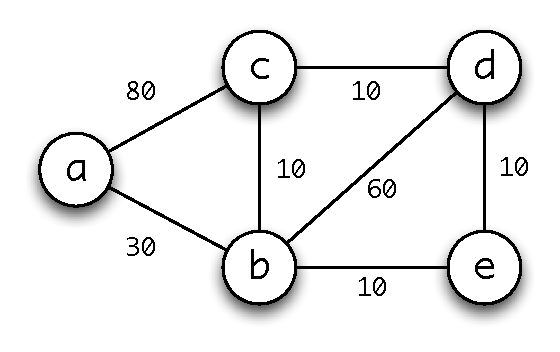
\epsfig{file=eps/flight-costs.eps,width=0.45\columnwidth}
\caption{Flight Map and Cost Between 5 Cities}
\label{fig:flight}
\end{figure}

\begin{figure}[tb]
\begin{lstlisting}[label=lst:tsell,caption=Ticket Seller's Agent. \texttt{[...]} denotes a list while \texttt{X[$i$]} is the $i$-th element of list \texttt{X}. \texttt{rand($m$)} returns a random integer between $0$ and $m$ (inclusive). \texttt{X.Y} denotes the concatenation of symbols so that \texttt{u.v} evaluates to \texttt{uv}.]
Ts = [[a,b,30],[a,c,80],[b,c,10],
      [b,d,60],[b,e,10],[c,d,10],[d,e,10]]
loop
  T = Ts[rand(6)]
  if rand(1) = 0
    |$\Out$|(ticket, T[0].T[1], T[2])
  else
    |$\Out$|(ticket, T[1].T[0], T[2])
|$\exit$|
\end{lstlisting}
\begin{lstlisting}[label=lst:tbuy,caption={Ticket Buyer's Agent. Both {\tt fly()} and {\tt try()} are defined using pattern matching on parameters. \texttt{[N:Ns]} denotes a list which has \texttt{N} as its head and \texttt{Ns} as its tail. Underscore (\texttt{\_}) matches anything in the context of pattern matching.}]
fly(X, X, Cash, V): arrived
fly(X, Y, Cash, V): Ns = unvisited_neighbors(X, V)
                    try(X, Ns, Y, Cash, V)

try(X, [N],    Y, Cash, V): buy(X, N, Y, Cash, V)
try(X, [N:Ns], Y, Cash, V): (buy(X, N, Y, Cash, V)
                            |$\oplus$|try(X, Ns, Y, Cash, V))
                            |$\cm$|

buy(X, N, Y, Cash, V):
  |$\In$|(ticket, X.N, |$\lambda x.x\le\texttt{Cash}$|) = (_, _, Cost)
  fly(N, Y, Cash - Cost, [N:V])

fly(a, e, 100, [a])
|$\exit$|
\end{lstlisting}
\vspace*{-5mm}
\end{figure}

\subsubsection*{Stock Trading (ST)}

In this example, we set up a mini stock market which follows the prices in the public exchange 
but is not openly available to the public. 
Traders can join the market at any time but their trades will not affect the public market.
Markets like this do exist in real life in the form of 
``Dark Pools''\cite{degryse2008shedding}  
which offers anonymous and private investors to
trade away from the public exachanges.

Our market starts with $N$ stocks, each has a fixed amount of shares dedicated for this market.
In general, each trader has a fixed amount of money in the beginning, 
and can buy (or sell) stocks from (or to) the market according to the public prices.
% Each trader also has a high watermark and a low watermark of cash.
% When the cash value is less than the low watermark (or greater than the high watermark), 
% the trader will keep selling (or buying) stocks in order to increase (or decrease) the cash value. 
% This strategy comes from real-world strategies where people want to control the risk.
% Different watermarks lead to different behaviors, and for this example, 
% the traders speculate to be either conservative or aggressive.
Listing \ref{lst:trader} shows the trader's agent program. 
Each trader trades several rounds until his cash value reaches the goal. 
For each round, the trader randomly picks a stock {\tt X}, buys it as much as possible, 
and waits for the price of {\tt X} to change. 
$\alpha$ is a value between 0 and 1 which indicates the profit/loss margin percentage. 
For example, if a trader buys {\tt X} at a price of {\tt P}, 
he sells it at a price of either higher than $(1+\alpha)\times{\tt P}$ (to profit)
or lower than $(1-\alpha)\times{\tt P}$ (to prevent further loss). 
Different $\alpha$ values lead to different trading behaviors, and for this example,
the traders speculate to be either 
conservative (smaller $\alpha$) or aggressive (larger $\alpha$).
Note that there is no atomicity guarantee between checking the price of a stock 
and actually buying it, which is also the behavior of a real market.
Also an intention to buy can be partially filled by the stock-serving agent
(see Listing \ref{lst:stock}).
The stock-serving agent also waits for price updating (i.e. {\tt (update, ...)})
from the public exchange in a realtime fashion. 

\begin{figure}[tb]
\begin{lstlisting}[label=lst:trader,caption={Trader's Agent. Numbers are irrelevant and just for illustration purposes.}]
Me     = unique_account_name
Stocks = [...]  // a list of stock names
Start  = 5000   // start with cash of $5000
Goal   = 5500   // the goal is to end up with $5500

trade(Cash, |$\alpha$|):
  X = Stocks[rand(N-1)]

  |$\Rd$|(price, X, _) = (_, _, P1)
  Q1 = |$\lfloor$|Cash / P1|$\rfloor$|
  |$\Out$|(buy, X, Q1, Me)
  |$\In$|(ack, Me, _, _) = (_, _, P2, Q2)
  C1 = Cash - P2 * Q2

  |$\Rd$|(price, X, |$\lambda x.x\ge(1+\alpha)\times{\tt P2}\lor x\le(1-\alpha)\times{\tt P2}$|)
  |$\Out$|(sell, X, Q2, Me)
  |$\In$|(ack, Me, _) = (_, _, P3)
  C2 = C1 + P3 * Q2

  if C2 < Goal
    trade(C2, |$\alpha$|)
  else
    |$\cm$|

trade(Start, 0.01) |$\oplus$| trade(Start, 0.05)
|$\exit$|
\end{lstlisting}
\begin{lstlisting}[label=lst:stock,caption=Stock-serving Agent. \texttt{P} is the current price of the stock while \texttt{Q} is the quantity of stocks available for sale.]
Me = unique_stock_name

serve(P, Q):
  case |$\In$|(_, Me, _, _)
    (update, _, NewPrc, _): |$\In$|(price, Me, _)
                            |$\Out$|(price, Me, NewPrc)
                            serve(NewPrc, Q)

    (buy, _, Q1, X): Q2 = min(Q1, Q)
                     |$\Out$|(ack, X, P, Q2)
                     serve(P, Q - Q2)
    
    (sell, _, Q2, X): |$\Out$|(ack, X, P)
                      serve(P, Q + Q2)

|$\Out$|(price, Me, Start_Price)
serve(Start_Price, Start_Quantity)
\end{lstlisting}
\vspace*{-6mm}
\end{figure}

\subsubsection*{Dining Philosophers (DP)}

% \begin{figure}[tb]
% \centering
% 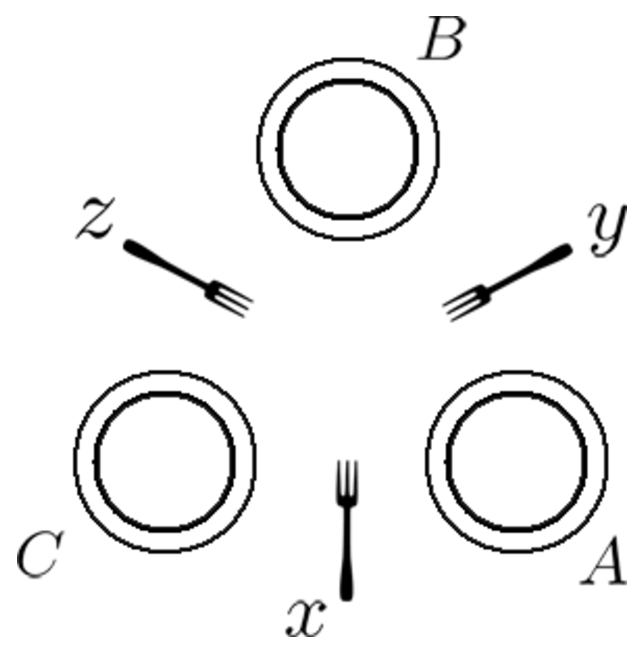
\epsfig{file=eps/dining.eps,width=0.3\columnwidth}
% \caption{Three Dining Philosophers Problem.
% $A,B,C$ are philosophers while $x,y,z$ are forks.}
% \label{fig:dining}
% \end{figure}

% \RY{can delete the figure. Listing 9 can be joined horizontally rather
% than vertically as now}

Consider the well-known ``Dining Philosophers Problem''
\cite{Dijkstra2002:Hierarchical} - there are three
philosophers $A$, $B$ and $C$, sitting around a dining table,
with three forks $x$, $y$ and $z$ between them.
This classic concurrency problem
shows that deadlock happens with certain sequences of acquiring the forks,
e.g., $A$ acquires $x$, $B$ acquires $y$ and then
$C$ acquires $z$. 
The classic solution to this problem is using a synchronization mechanism 
such as a counting semaphore, imposing a partial order on acquiring the forks, 
or requiring one philosopher to be asymmetric.
However, such kind of solution requires additional constraints to the problem. 
%
In this example, the speculation framework offers an alternative
solution which is purely based on the definition of the problem.
We extend the problem to $N$ dining philosophers 
sitting around a table with $N$ forks.
For simplicity, each philosopher has a unique index ranging from $0$ to $N-1$. 
Listing \ref{lst:dpinit} shows the initialization of data stores 
for dining philosophers.
Listing \ref{lst:dp} shows the agent program for dining philosophers.
\texttt{my\_index()} returns the index of the current philosopher.

\begin{figure}[tb]
\begin{lstlisting}[label=lst:dpinit,caption=Dining Philosophers (initialization)]
for I = 0 to N-1
  |$\Out$|(fork,I)
|$\exit$|
\end{lstlisting}
\begin{lstlisting}[label=lst:dp,caption={Dining Philosophers. \texttt{\%} denotes the modulo operation. {\tt ;} separates multiple statements in one line. $\Out$ is non-blocking in the tuple space data model, so we don't need choices for putting back forks.}]
L = my_index(); R = (L+1) % N
(|$\In$|(fork,L); |$\In$|(fork,R)) |$\oplus$| (|$\In$|(fork,R); |$\In$|(fork,L))
|$\cm$|
|$\Out$|(fork,L); |$\Out$|(fork,R)
|$\exit$|
\end{lstlisting}
\shrink
\shrink
\end{figure}

By using such kind of speculation, it can be guaranteed that 
there is always one world where nobody deadlocks. 
For example, assume $N=3$, the combination of the choices from three philosophers 
theoretically creates eight worlds as in Figure \ref{fig:diningrun} 
(though in practice some of the worlds may never be there due to pruning).

\begin{figure}
\centering\small
\Tree[.$\oplus_A$
    [.$\oplus_{B_1}$
        [.$\oplus_{C_1}$
            {$A\compact:-x$ \\ $\quad-y$ \\ $B\compact:-y$ \\ $\quad-z$ \\ $C\compact:-z$ \\ $\quad-x$ \\ $(w_1)$}
            {\bk$A\compact:-x$ \\ \bk$\quad-y$ \\ \bk$B\compact:-y$ \\ \bk$\quad-z$ \\ \bk$C\compact:-x$ \\ \bk$\quad-z$ \\ $(w_2)$}
        ][.$\oplus_{C_2}$
            {$A\compact:-x$ \\ $\quad-y$ \\ $B\compact:-z$ \\ $\quad-y$ \\ $C\compact:-z$ \\ $\quad-x$ \\ $(w_3)$}
            {\bk$A\compact:-x$ \\ \bk$\quad-y$ \\ \bk$B\compact:-z$ \\ \bk$\quad-y$ \\ \bk$C\compact:-x$ \\ \bk$\quad-z$ \\ $(w_4)$}
        ]
    ][.$\oplus_{C_3}$
        [.$\oplus_{B_2}$
            {$A\compact:-y$ \\ $\quad-x$ \\ $B\compact:-y$ \\ $\quad-z$ \\ $C\compact:-z$ \\ $\quad-x$ \\ $(w_5)$}
            {\bk$A\compact:-y$ \\ \bk$\quad-x$ \\ \bk$B\compact:-z$ \\ \bk$\quad-y$ \\ \bk$C\compact:-z$ \\ \bk$\quad-x$ \\ $(w_6)$}
        ][.$\oplus_{B_3}$
            {$A\compact:-y$ \\ $\quad-x$ \\ $B\compact:-y$ \\ $\quad-z$ \\ $C\compact:-x$ \\ $\quad-z$ \\ $(w_7)$}
            {\bk$A\compact:-y$ \\ \bk$\quad-x$ \\ \bk$B\compact:-z$ \\ \bk$\quad-y$ \\ \bk$C\compact:-x$ \\ \bk$\quad-z$ \\ $(w_8)$}
        ]
    ]
]
\caption{Three Dining Philosophers Problem (tree of choices). Minus sign ($-$) denotes taking the fork. Deadlock only happens in $w_1$ and $w_8$.}
\label{fig:diningrun}
\shrink
\end{figure}

There are many practical algorithms and applications (e.g., 2-phase locking)
that are special cases or extensions of the Dining Philosopher Problem (DPP). 
So we generalize DPP as follows.
\begin{definition}[Generalized Dining Philosopher Problem]
Given a set of resources $R$ which are available at the beginning, 
$n$ agents each interested in a subset of resources 
$R_i\subseteq R (1\le i\le n)$, and each agent is a two-phase process:
  \begin{enumerate}
    \item In the \emph{acquisition phase} the agent consumes every resource $r\in R_i$ in any order;
    \item In the \emph{release phase} the agent puts back every resource $r\in R_i$ in any order.
  \end{enumerate}
  $R_i$'s may overlap so the scheduler may produce a schedule which can cause deadlock 
among the agents.
\end{definition}

\begin{theorem} Generalized Dining Philosopher Problems do not deadlock 
using speculative nondeterminism.
\end{theorem}
\begin{proof}[Proof sketch]
% first show there is always a solution
First, we construct a combination of choices which will never deadlock. 
Fix an ordering of the elements in $R$, for example $r_1,r_2,\dots,r_m$ where $m=|R|$. 
For any agent $i$, it consumes $R_i$ in this fixed order. 
Then there will be races instead of deadlocks because there will not be the 
case that agent $i$ consumes $r_x$ and waits for $r_y$, and agent $j$ consumes
$r_y$ and waits for $r_x$ ($x<y$ and $y<x$ cannot be true at the same time). 
% then show the solution will not be pruned
Then it can be shown this combination will not be pruned by commits in an 
eventually blocking world due to the commit semantics described in rule \ref{rule:cm}. 
\end{proof}


\begin{figure}[ht!]
\centering
% TODO: use a tabular{cr} to format better
\flushright\fbox{Entrance transition: $T\|a\Longrightarrow T'$}
\[
  \tag{\sc Entrance1}\label{rule:entrance1}
  \langle A,D,S\rangle \| a \Longrightarrow \langle A+[a],D,S\rangle
\]
\[
  \tag{\sc Entrance2}\label{rule:entrance2}
  T_1\oplus_k T_2 \| a \Longrightarrow (T_1 \| a)\oplus_k (T_2 \| a)
\]
\flushright\fbox{Tree transition: $T\To T'$}
\[
  \tag{\sc Swap}\label{rule:swap}
  T_1\oplus_k T_2 \To T_2\oplus_k T_1
\]
\[
  \tag{\sc DataOp}\label{rule:dataop}
  \frac
  {A[k]=d.e:f \qquad D\vdash d \qquad \langle t,D'\rangle=\psi(d,D)}
  {\langle A,D,S\rangle \To \langle A[k\mapsto t.e:f], D', S\rangle}
\]
\[
  \tag{\sc Choice}\label{rule:choice}
  \frac
  {\begin{matrix}
    A[k]=(e_1\oplus e_2).e:f \\
    T_1=\langle A[k\mapsto e_1.e:f],D,S\rangle \\
    T_2=\langle A[k\mapsto e_2.e:f],D,S\rangle
   \end{matrix}}
  {\langle A,D,S\rangle \To T_1\oplus_k T_2}
\]
\[
  \tag{\sc Cm}\label{rule:cm}
  \frac
  {A[k]=\cm.e:f}
  {\langle A,D,S\rangle\oplus_k T \To \langle A[k\mapsto e:f],D,S\rangle}
\]
\[
  \tag{\sc Cu}\label{rule:cu}
  \frac
  {A[k]=\cu.e:f}
  {\langle A,D,S\rangle\oplus_k T \To T}
\]
\[
  \tag{\sc Exit1}\label{rule:exit1}
  \frac
  {A[k]=\exit.e :f \qquad s=\langle k,f(D)\rangle}
  {\langle A,D,S\rangle \To \langle A[k\mapsto\exiting],D,S\cup\{s\}\rangle}
\]
\[
  \tag{\sc Exit2}\label{rule:exit2}
  \frac
  {\begin{matrix}
    \forall w\in leaves(T): exiting(w,k) \land v = exitv(w,k)
   \end{matrix}}
  {T \To exit(T,k)}
\]
\[
  \tag{\sc Collapse}\label{rule:collapse}
  \frac
  {\begin{matrix}
    w \in leaves(T) \\
    \forall k: exiting(w,k) \lor exited(w,k)
   \end{matrix}}
  {T \To w}
\]
\flushright\fbox{Local computation transition: $e\computes e'$}
%\begin{align*}
\[
\begin{array}{llll}
  e &\computes op.e' \hspace*{5mm} &
  e &\computes \epsilon \\
  t.e &\computes e' &
  e_1.e_2 &\computes e_1'.e_2 \\
\end{array}
\]
%%  \epsilon.e &\computes e
%\end{align*}
\flushright\fbox{Helper functions}
\begin{gather*}
  \frac
  {T = T_1\oplus_k T_2}
  {leaves(T) = leaves(T_1)\uplus leaves(T_2)} \\
  leaves(w) = \lbb w\rbb \\
  \frac
  {w=\langle A,D,S\rangle \qquad \langle k,v\rangle\in S}
  {exitv(w,k) = v} \\
  \frac
  {w=\langle A,D,S\rangle}
  {exiting(w,k) = (A[k]=\exiting)} \\
  \frac
  {w=\langle A,D,S\rangle}
  {exited(w,k) = (A[k]=\exited)} \\
  \frac
  {T = T_1\oplus_i T_2}
  {exit(T,k) = exit(T_1,k)\oplus_i exit(T_2,k)} \\
  \frac
  {w=\langle A,D,S\rangle}
  {exit(w,k) = \langle A[k\mapsto\exited],D,S\rangle}
\end{gather*}
\caption{Semantics of the Speculation Language.
$[\dots]$ denotes a list,
$A[k]$ is the $k$-th element in list $A$, and
$A[k\mapsto x]$ denotes the updating of the $k$-th element to $x$.}
\label{fig:semantics}
\end{figure}

\subsection{Semantics}\label{sec:semantics}

The semantics of the speculation language is 
given in \figref{fig:semantics}. 

\paragraph*{Entrance}
New agents can dynamically enter the system at any time.
\ref{rule:entrance1} and \ref{rule:entrance2} the addition of
a new agent $a$ to the system (denoted $\|$). The Plus sign ($+$) 
denotes list concatenation. The whole tree is recursively traversed and $a$ is appended to the agent list in every world. 

\paragraph*{Choice Symmetry}
\ref{rule:swap} shows that the two branches of an interior node in the tree are treated equally.

\paragraph*{Data Operation}
An agent wants to execute operation $d$ on the data store $D$
(see \ref{rule:dataop}).
This transition first has to meet condition $D\vdash d$. 
The effect of $d$ on data store $D$ is defined by
the transition function $\psi$ in the data model and it only
affects the current world having store $D$
without affecting other worlds in the tree.
The result of $d$ is denoted is $t$ and provided to the remaining local 
computation $e$ as a parameter (denoted by the special syntax $t.e$). 
$t.e$ is not processed by the speculation framework, but 
activates the local computation $e$ and will eventually transform to another 
local computation $e'$ (i.e. $t.e\computes e'$). 

\paragraph*{Local Computation}
The local computation transition is simply a placeholder for
the semantics of the actual computation in the host language.
As that is orthogonal to our semantics, the details are left
unspecified. There is one special operation, $t.e$, which applies
the result of a data operation $t$ to some local computation $e$.
For example, it might be to store $t$ in a variable in the host language.
% \KZ{The following may need to be changed:\\
% We shall omit the details of the language in which 
% local computations are expressed and just assume that
% there exist a local computation transition $\computes$.
% From the perspective of the speculation framework, 
% the only thing that matters is the operation $op$ 
% produced by a local computation. 
% As shown in \figref{fig:semantics}, 
% a local computation $e$ transforms to $op.e'$ to 
% execute $op$ under the framework, or to $\epsilon$ to 
% finish execution. 
% After a data operation which reads something from the data store,
% a data item $t$ in the store is returned to the local computation $e$, 
% and further transforms to a new local computation $e'$, which is 
% $e$ parameterized by $t$. 
% $e_1.e_2$ denotes sequential execution of $e_1$ and $e_2$. 
% After $e_1$ transforms to $\epsilon$, $e_2$ starts execution 
% ($\epsilon.e\computes e$).
% }

\paragraph*{Choice and Commit}
Speculative nondeterminism provides for the creation and subsequent
pruning of choices. 
\ref{rule:choice} fires if an agent is reduced to a choice $(e_1\oplus e_2).e$, 
and it consumes the choice construct in the agent to split the current world into two
(i.e. $T_1$ and $T_2$). 
Section \ref{sec:commit} discusses further the ramifications of commit,
here, we start with first describing what the commit rules do.
When the $k$-th agent executes $\cm$ in a leaf world of the tree structure, 
as shown in rule \ref{rule:cm}, the other side of the choice (i.e. $T$) is pruned
only if the current choice node is $\oplus_k$. 
Similarly, $\cu$ is used where the agent wants to explicitly gives up the current choice branch,
so the current side of the choice is pruned, 
as shown in rule \ref{rule:cu}. 
$\cm$ and $\cu$ are symmetric and both of them are {\em commit} operators.
Commit of the $k$-th agent can only be executed in a world with $\oplus_k$ as its parent,
and it is blocking when the parent node is not $\oplus_k$.
%which makes the commit more localized and less aggressive. 
% This form of commit semantics is therefore known as {\em localized commit}.
%With this commit semantics, it only affects a small fraction of the whole tree. 
%Also it is possible to make pruning decisions locally, which makes it efficient. 

\paragraph*{Exit}
In general, a single agent will have many versions of itself executing
in all the multiple virtual worlds.
Thus, if it were simply to exit from all the worlds on the first
$\exit$ operation, this could lead to some form of data inconsistency.
We deal with this using the exit function $f$ specified by each agent which
allows an agent-specific consistency condition to be used.
Note that different agents may be interested in different aspects of the data store. 
When an agent exits, all the worlds should look the same from the perspective of that agent. 
However, another agent may not consider the worlds to be the 
same since it can have a different exit function. 
This also means that an agent properly exiting is only achieved when
the consistency requirement is obtained.

Rule \ref{rule:exit1} and \ref{rule:exit2} shows the exit semantics. 
\ref{rule:exit1} shows the case when an {\em instance} 
of the $k$-th agent reaches $\exit$ in a world. 
In this case, the exit function $f$ is applied to the current data store $D$ and a {\em snapshot} 
is created and added to $S$. 
 
The exit function $f$ takes a data store as input, and returns an integer as the evaluated result. 
The data store is just the one associated with the current world. 
According to the data store, the exit function is expected to produce an integer 
which can be a 0/1 indicator, a heuristic value, or an encoding of more complicated mathematical objects. 
For example, in the simplest case, $f(d)\equiv 1$ allows the agent to exit without any condition 
as long as it completes execution of all the operations in the program. 
The ability to return an integer provides more flexibility and enables 
complex exiting logic to be embedded in this exit function.

While taking a snapshot, 
the agent in that world switches to a special state $\exiting$.
\ref{rule:exit2} checks all the worlds in the tree. Only if (i) the $k$-th agent has 
switched to $\exiting$ state in all the worlds, and (ii) the exit value $v$ of the $k$-th agent 
is {\em identical} across all the worlds, 
then the $k$-th agent can exit from the worlds at the same time. 
For \ref{rule:exit2}, the exit value $v$, which can be thought of as the return value from
the speculative computation, will be eventually provided to 
a local computation $\tilde e$
which is completely outside the system of virtual worlds, 
and has no more speculation and data store operations. 
The idea of this type of consistent exit across all worlds is analogous
algebraic factorization, i.e.
$ab + ac = a(b+c)$.

\paragraph*{Collapse}
Note that commit is optional in an agent program, so the agents can 
let the tree expand without pruning, and finally leave the tree 
without reducing to one world. 
Therefore some agents may never exit due to the inconsistency of some worlds, 
even if all the agents have finished execution.
\ref{rule:collapse} handles this case 
to let these agents exit as well as to reclaim system resources. 
The system could employ a global collapse rule to pick any world where 
all agents have completed execution and reduce the tree to one world.
For \ref{rule:collapse}, the exit value for every agent $k$ is also returned in this way.
$\tilde e$ can make use of the exit value to extract what the agent concerns. 
%\KZ{Need to say exit is implicit if it's not added to the program?}

\paragraph*{Helper Functions}
We also define a set of helper functions to simplify the semantics. 
\begin{description}
\item[$leaves(T)$] returns a multi-set of the leaf worlds in tree $T$. 
\item[$exitv(w,k)$] retrieves the exit value, i.e. the evaluation result of the exit function, of the $k$-th agent in world $w$.
\item[$exiting(w,k)$] is a predicate indicating whether the $k$-th agent in world $w$ is in the special state of $\exiting$.
\item[$exited(w,k)$] is a predicate indicating whether the $k$-th agent in world $w$ is in the special state of $\exited$.
\item[$exit(T,k)$] switches the $k$-th agent in all the worlds in $T$ to the special state of $\exited$.
\end{description}

\subsection{More on Commit}\label{sec:commit}
Commit is a special and important operation in speculative nondeterminism because:
(i) it gives the agent the power to specify preferences among different choices,
e.g., in Listing \ref{lst:intro-commit-sleep}; 
(ii) it prunes some of the virtual worlds to make it easier for agents to exit
because the fewer remaining worlds means easier consistency checks,
and thus it improves the responsiveness and overall throughput of the system;
(iii) by pruning worlds, it also reclaims precious system resources such as
memory and CPU cycles, which is critical to the viability of the multi-world 
speculation , even though the naive combinatorial problem space is exponential and
prohibitive.

However, it is also important to understand that whenever commit is used and
pruning is done, potential solutions can be pruned away, and deadlock or blocking
may arise as a result. So from the system point of view, we design a commit
semantics that is {\em localized} and less aggressive because the scope of the pruning
is restricted to be of height 1 only and affects only a small fraction of
the whole tree (see Rule \ref{rule:cm}). This commit semantics is also
more efficient because pruning decisions are made locally. There are of course
other possible commit semantics \cite{JaffarYZ07} which are more eager in pruning. 
For example, one type of commit requires agent $T$ to commit in all left or right
subtree rooted at $\oplus_T$. These are either too aggressive and lose 
too many solutions or require coordination
among various worlds which is more costly to execute in practice.

From the programmer's point of view, she should use commit with care, knowing that
without commit, the multi-world space grows very quickly and the program probably
cannot scale, but with commit, the program could potentially lose valuable solution.
It makes more sense to put commit later rather than early in the choice. 
If one must put a commit in the middle of a sequence of operations like
$op_1.op_2.\cm.op_3.op_4$, she should ensure that the remaining operations
after $\cm$, i.e., $op_3$ and $op_4$, are not likely to block, 
e.g., when they are local computations.

%The commit semantics described in Section \ref{sec:semantics} 
%is called {\em localized commit} as it restricts
%the scope of pruning to be of height 1 only.  
%%$\cm$ by agent $X$ cannot
%%prune until the direct parent of the committed world is $\oplus_X$.
%%$\cu$ kills the current world immediately without coordination with other worlds.
%Besides localized commit, there is a number of other possible commit
%semantics \cite{JaffarYZ07}.
%They differ in their eagerness to prune the worlds.
%They are ordered roughly from the most eager to the most conservative:
%{\em absolutely eager commit}, {\em eager commit}, {\em coordinated commit}, 
%{\em late commit} and {\em no commit}. 
%


